% =============================================================================
% isimustangerp/latex/main.tex — Perfil de Proyecto de Grado
% Diseño e Implementación de un Sistema ERP Modular para ISI Mustang Bolivia
%
% Motor requerido: XeLaTeX
%   Compilar con: latexmk -xelatex main.tex  (ejecutar desde esta carpeta)
%
% Dependencias:
%   univalle-perfil.cls  — enlace simbólico a ../../formato/univalle-perfil.cls
%   ../../imagenes/      — imágenes (logo en carátula)
%   referencias.bib      — base bibliográfica local
% =============================================================================

\documentclass{univalle-perfil}

\graphicspath{{../../}}
\addbibresource{referencias.bib}

\usepackage{tikz}
\usepackage{pgfplots}
\pgfplotsset{compat=newest}
\usetikzlibrary{shapes.geometric, positioning, arrows.meta}

% -----------------------------------------------------------------------------
% METADATOS DE LA CARÁTULA
% -----------------------------------------------------------------------------
\universidad{Universidad Privada del Valle}
\facultad{Facultad de Informática y Electrónica}
\carrera{Carrera de Licenciatura en Ingeniería de Sistemas}
\tituloTrabajo{Diseño e Implementación de un Sistema ERP Modular para la Gestión Integral de Proyectos de Ingeniería: Caso ISI Mustang Bolivia}
\modalidad{Proyecto de Grado}
\tituloOptar{Licenciatura en Ingeniería de Sistemas}
\postulante{[Nombre del Postulante]}
\tutor{[Nombre del Tutor]}
\ciudad{Santa Cruz}
\pais{Bolivia}
\anio{2026}

% =============================================================================
\begin{document}

% --- Carátula ----------------------------------------------------------------
\makecaratula

% --- Índices -----------------------------------------------------------------
\pagenumbering{gobble}
\tableofcontents
\listoffigures

% --- Contenido principal -----------------------------------------------------
\pagenumbering{arabic}

% =============================================================================
% 1. INTRODUCCIÓN
% =============================================================================
\section{Introducción}

Los sistemas de planificación de recursos empresariales (ERP) constituyen hoy la columna vertebral de la gestión operativa en organizaciones de todos los tamaños. Desde su aparición en la década de 1990, estos sistemas han evolucionado hasta convertirse en plataformas integradas que centralizan datos, automatizan procesos y proporcionan visibilidad en tiempo real sobre la operación del negocio \parencite{monk2012}.

ISI Mustang Bolivia es una empresa de consultoría e ingeniería industrial que gestiona proyectos para clientes en sectores de industria, minería y construcción en Santa Cruz de la Sierra. Su operación diaria involucra la coordinación de equipos de trabajo, el control de costos por proyecto, la gestión de horas hombre, el manejo de requisiciones de compra, viáticos y el seguimiento financiero de cada contrato activo. Sin embargo, el sistema de gestión con el que opera actualmente ha cumplido su ciclo de vida útil, generando limitaciones técnicas documentadas que impactan directamente en la eficiencia operativa de la empresa.

A nivel global, las soluciones ERP dominantes como SAP, Oracle ERP Cloud y Odoo representan alternativas con alto costo de licenciamiento y elevada complejidad de implementación, lo que las hace poco adecuadas para empresas medianas latinoamericanas con procesos de negocio específicos y recursos limitados para adaptación. En el contexto boliviano, la alternativa más común es continuar operando con hojas de cálculo o sistemas desarrollados internamente con tecnología obsoleta, lo que genera ineficiencias operativas documentadas y riesgo de pérdida de información crítica del negocio.

El presente trabajo propone el diseño e implementación de un sistema ERP modular, construido sobre tecnologías modernas de código abierto, específicamente adaptado a los procesos operativos de ISI Mustang Bolivia. El sistema integra siete módulos funcionales que cubren el flujo de negocio completo: desde la autenticación y el control de acceso hasta el control presupuestario por proyecto, pasando por la gestión de propuestas comerciales, horas de trabajo y planilla de personal. El entregable principal es un sistema funcional construido en fases incrementales y validado mediante pruebas con usuarios reales de la empresa.

% =============================================================================
% 2. ANTECEDENTES DEL PROBLEMA
% =============================================================================
\section{Antecedentes del Problema}

ISI Mustang Bolivia gestiona múltiples proyectos simultáneamente, cada uno con su propio presupuesto, equipo asignado, requisiciones de compra y ciclo de certificación mensual. La información de cada proyecto se encuentra dispersa en el sistema actual, sin integración real entre los módulos de gestión de personal, control financiero y pipeline comercial. Esto genera ineficiencias en la toma de decisiones gerenciales, duplicación de trabajo administrativo y riesgo de pérdida de información crítica del negocio.

El análisis del entorno operativo actual se sintetiza en el Cuadro 2.1 mediante un análisis FODA, que identifica las fortalezas y debilidades del contexto actual, así como las oportunidades y amenazas que determinan el espacio de solución del problema.

\begin{table}[H]
\centering
\caption{Análisis FODA del entorno operativo de ISI Mustang Bolivia.}
{\renewcommand{\arraystretch}{1.5}
\begin{tabular}{|p{0.44\textwidth}|p{0.44\textwidth}|}
\hline
\textbf{Fortalezas} & \textbf{Oportunidades} \\
\hline
$\bullet$~Empresa con procesos de negocio consolidados y usuarios con experiencia operativa documentada.\newline
$\bullet$~Infraestructura tecnológica disponible para el despliegue del nuevo sistema.\newline
$\bullet$~Artefactos de ingeniería preexistentes: ERD completo, FRDs de tres módulos y diagramas de proceso.
&
$\bullet$~Disponibilidad de frameworks modernos de código abierto (NestJS, PostgreSQL) con soporte activo de la comunidad.\newline
$\bullet$~Ausencia de soluciones ERP especializadas para empresas de ingeniería de proyectos en Bolivia.\newline
$\bullet$~Demanda real de la empresa anfitriona, que actúa como organización patrocinadora con usuarios disponibles para validación.
\\
\hline
\textbf{Debilidades} & \textbf{Amenazas} \\
\hline
$\bullet$~Sistema actual sin trazabilidad de cambios ni notificaciones automáticas en flujos de aprobación.\newline
$\bullet$~Ausencia de vista financiera consolidada: la gerencia debe navegar módulo por módulo para obtener métricas de cada proyecto.\newline
$\bullet$~Desconexión entre pipeline comercial y ejecución operativa de proyectos.
&
$\bullet$~Resistencia al cambio de parte de usuarios habituados al sistema anterior.\newline
$\bullet$~Modificaciones de requerimientos durante el desarrollo que amplíen el alcance acordado.\newline
$\bullet$~Dependencia del acceso continuo a ISI Mustang para relevamiento, validaciones y pruebas de aceptación.
\\
\hline
\end{tabular}}
\fuente{Elaboración propia, 2026.}
\end{table}

A nivel nacional, no existen soluciones ERP especializadas accesibles para empresas de consultoría e ingeniería de proyectos bolivianas de tamaño medio. Las alternativas internacionales disponibles —SAP, Oracle ERP Cloud y Odoo— presentan barreras de costo de licenciamiento y complejidad de implementación que las hacen inviables para organizaciones con recursos limitados para adaptación \parencite{monk2012}.

\subsection{Planteamiento del Problema}

ISI Mustang Bolivia gestiona múltiples proyectos simultáneamente con información dispersa en un sistema legacy que no permite incorporar nuevas funcionalidades, carece de trazabilidad en los cambios de estado de proyectos y propuestas, no notifica automáticamente a los responsables en los flujos de aprobación, y no ofrece una vista consolidada del rendimiento financiero de todos los proyectos activos. Los problemas identificados son los siguientes: ausencia de registro auditable de cambios; flujos de aprobación sin notificaciones que generan demoras operativas que impactan la ejecución de proyectos; inexistencia de un tablero que consolide márgenes reales, desvíos de costos y porcentaje de avance en una sola pantalla; desconexión formal entre el pipeline comercial y la ejecución de proyectos; y un cálculo de costos deficiente que requiere la combinación manual de información entre múltiples pantallas sin mecanismo de cierre de período contable. ¿En qué medida el diseño e implementación de un sistema ERP modular, utilizando una arquitectura de dominio separado sobre NestJS y PostgreSQL, puede resolver las limitaciones de integración, trazabilidad y control financiero del sistema de gestión actual de ISI Mustang Bolivia?

\subsection{Objeto de Estudio}

Los procesos de gestión operativa y financiera de proyectos de ingeniería en ISI Mustang Bolivia: la coordinación de equipos de trabajo, el control de costos por proyecto, la gestión de horas hombre, el seguimiento financiero de contratos activos y el pipeline comercial de propuestas, tal como se realizan actualmente en el sistema de gestión vigente.

% =============================================================================
% 3. OBJETIVOS
% =============================================================================
\section{Objetivos}

\subsection{Objetivo General}

Diseñar e implementar un sistema ERP modular para la gestión integral de proyectos de ingeniería que integre los módulos de autenticación y control de acceso, gestión de centros de costo, proyectos y clientes, propuestas comerciales, horas por proyecto, planilla de personal y costos, y presupuestos por proyecto, resolviendo las limitaciones de trazabilidad, integración y control financiero del sistema actual de ISI Mustang Bolivia.

\subsection{Objetivos Específicos}

\begin{itemize}
    \item Relevar y documentar los procesos de negocio actuales de ISI Mustang Bolivia mediante entrevistas estructuradas con usuarios clave y análisis del sistema existente, produciendo especificaciones funcionales por módulo.
    \item Diseñar el modelo de datos del sistema ERP sobre PostgreSQL, garantizando integridad referencial, trazabilidad completa de cambios y control de períodos contables mediante restricciones a nivel de base de datos.
    \item Implementar el módulo de Autenticación y Control de Acceso con gestión de roles y permisos granulares, permitiendo que cada usuario acceda únicamente a las funcionalidades correspondientes a su rol en el sistema.
    \item Implementar el módulo de Gestión de Centros de Costo, que actúa como entidad central de imputación de todos los movimientos económicos del sistema.
    \item Implementar el módulo de Proyectos y Clientes, incluyendo el historial auditable de cambios de estado y la vinculación formal entre proyectos, centros de costo y clientes.
    \item Implementar el módulo de Propuestas Comerciales con dashboard de pipeline comercial y activación automática de proyectos al ganar una propuesta.
    \item Implementar los módulos de Gestión de Horas por Proyecto, Planilla de Personal y Costos, y Presupuestos por Proyecto, cubriendo el flujo de control financiero desde la imputación de tiempo hasta el control presupuestario.
    \item Validar el sistema implementado mediante pruebas funcionales por módulo y pruebas de aceptación con usuarios reales de ISI Mustang Bolivia, verificando que los flujos de trabajo documentados se comportan según lo especificado.
\end{itemize}

% =============================================================================
% 4. JUSTIFICACIÓN
% =============================================================================
\section{Justificación}

El presente proyecto se justifica por la existencia de un problema operativo concreto y verificable en ISI Mustang Bolivia, cuya solución requiere la aplicación integrada de conocimientos de ingeniería de software, diseño de bases de datos y arquitectura de sistemas. El proyecto cubre el ciclo completo de desarrollo de software en un contexto real de aplicación, lo que lo convierte en un aporte simultáneamente práctico, técnico y académico.

\subsection{Justificación Práctica}

El sistema propuesto reemplaza directamente el sistema de gestión actual de ISI Mustang Bolivia, resolviendo problemas operativos concretos que afectan la eficiencia diaria de la empresa. Al finalizar el proyecto, ISI Mustang contará con flujos de aprobación con notificaciones automáticas por correo electrónico, un pipeline comercial con activación automática de proyectos al ganar una propuesta, control de horas y costos de personal por proyecto con cierre de períodos que garantiza la integridad contable, y un tablero gerencial consolidado con métricas financieras en tiempo real. La empresa actúa como organización anfitriona del proyecto, proporcionando acceso a usuarios reales, procesos de negocio documentados y retroalimentación directa durante el desarrollo.

\subsection{Justificación Técnica}

El proyecto aplica y valida en un contexto real un conjunto de decisiones arquitectónicas que son objeto de estudio en ingeniería de software. La arquitectura monolítica modular con separación por dominios permite escalar el sistema a microservicios en el futuro sin reescribir la base, y representa una alternativa documentada con menor complejidad operacional que los microservicios desde el inicio \parencite{newman2021}. La implementación de reglas de negocio críticas directamente en la base de datos mediante políticas de seguridad a nivel de fila y triggers de PostgreSQL garantiza que las restricciones se apliquen independientemente del mecanismo de acceso al dato, incluso ante errores en la capa de aplicación \parencite{postgresql2024}. El motor de aprobaciones unificado y reutilizable entre todos los tipos de solicitudes del sistema evita la duplicación de lógica de negocio y facilita la auditoría centralizada.

\subsection{Justificación Académica}

La ingeniería de sistemas enfrenta el desafío constante de trasladar conceptos teóricos a soluciones funcionales en contextos reales. Este proyecto cubre el ciclo completo de desarrollo de software: relevamiento de requerimientos, análisis y modelado, diseño arquitectónico, implementación, pruebas y puesta en producción \parencite{sommerville2015}. Cada etapa genera artefactos documentables —FRDs, ERD, diagramas de arquitectura, resultados de pruebas— que constituyen evidencia académica del proceso. Adicionalmente, el proyecto aporta al conocimiento local un caso de estudio sobre el diseño de sistemas ERP para empresas de ingeniería de proyectos en Bolivia, un segmento escasamente documentado en la literatura técnica nacional.

% =============================================================================
% 5. DELIMITACIÓN DE LA INVESTIGACIÓN
% =============================================================================
\section{Delimitación de la Investigación}

\subsection{Temática}

La investigación se delimita al diseño e implementación de un sistema ERP modular orientado a la gestión integral de proyectos de ingeniería, abarcando los módulos de autenticación y control de acceso, gestión de centros de costo, proyectos y clientes, propuestas comerciales, gestión de horas por proyecto, planilla de personal y costos, y presupuestos por proyecto. El proyecto no abarca los módulos de requisiciones y compras, viáticos y movilidad, certificación planificada, tablero de comando gerencial, visualizador de consultas ni repositorio de reportes, que quedan definidos como trabajo futuro dependiente de los módulos implementados en este proyecto. El diseño del modelo de datos incluye las entidades necesarias para estos módulos futuros, garantizando que la arquitectura soporte la evolución del sistema.

\subsection{Espacial}

La investigación se desarrolla en la ciudad de Santa Cruz de la Sierra, Bolivia, tomando como organización anfitriona a ISI Mustang Bolivia. Las actividades de relevamiento de requerimientos, observación de procesos operativos y pruebas de aceptación con usuarios se realizan en las instalaciones de la empresa. Aunque el sistema puede adaptarse a otras empresas de consultoría e ingeniería de proyectos, los resultados de esta investigación se interpretan dentro del contexto operativo específico de ISI Mustang Bolivia.

\subsection{Temporal}

La investigación se desarrolla durante la gestión 2026, en un período estimado de veinticuatro semanas comprendidas entre el inicio del relevamiento formal y la entrega del documento final de tesis. Los resultados se limitan al estado de las tecnologías disponibles durante dicho período, particularmente en lo referente a NestJS versión 10, PostgreSQL versión 13 o superior, React versión 18, Prisma versión 5 y las herramientas de infraestructura de desarrollo utilizadas.

% =============================================================================
% 6. PROPUESTA DE SOLUCIÓN AL PLANTEAMIENTO DEL PROBLEMA
% =============================================================================
\section{Propuesta de Solución al Planteamiento del Problema}

El sistema propuesto es una plataforma ERP modular construida sobre una arquitectura monolítica modular con separación por dominios funcionales, implementada en NestJS con TypeScript para el backend, React con TailwindCSS para el frontend, y PostgreSQL como base de datos relacional con Prisma como ORM y gestor de migraciones. El sistema integra siete módulos funcionales que cubren el flujo de negocio completo de extremo a extremo: Cliente → Propuesta Comercial → activación automática al ganar la propuesta → Proyecto → Centro de Costo → imputación de Horas y Costos de Personal → control de Presupuesto.

\begin{table}[H]
\centering
\caption{Módulos del sistema ERP y descripción funcional.}
{\renewcommand{\arraystretch}{1.4}
\begin{tabular}{|p{0.06\textwidth}|p{0.28\textwidth}|p{0.55\textwidth}|}
\hline
\textbf{Mod.} & \textbf{Nombre} & \textbf{Funcionalidad principal} \\
\hline
M1 & Autenticación y Control de Acceso & Login, gestión de roles y permisos granulares, tokens de sesión JWT \\
\hline
M2 & Gestión de Centros de Costo & CRUD de centros de costo tipo Proyecto y Estructura, jerarquía de imputación \\
\hline
M3 & Proyectos y Clientes & CRUD de clientes y proyectos, historial auditable de cambios de estado \\
\hline
M4 & Propuestas Comerciales & Pipeline comercial, KPIs, activación automática de proyectos al ganar \\
\hline
M5 & Gestión de Horas por Proyecto & Grilla mensual de carga de horas, clasificación por actividad, flujo de aprobación \\
\hline
M6 & Planilla de Personal y Costos & Costo empresa por persona/mes, distribución proporcional a horas imputadas \\
\hline
M7 & Presupuestos por Proyecto & Categorías de presupuesto, doble vista Seguimiento vs.\ Publicado, horizonte multi-año \\
\hline
\end{tabular}}
\fuente{Elaboración propia, 2026.}
\end{table}

El diseño arquitectónico del sistema sigue los principios de la arquitectura limpia \parencite{martin2017}: cada módulo NestJS encapsula su propia lógica de dominio, exponiendo una interfaz pública que oculta los detalles de implementación. Las reglas de negocio críticas —en particular el control de períodos contables cerrados— se implementan a nivel de base de datos PostgreSQL, garantizando su aplicación independientemente del mecanismo de acceso al dato.

\begin{figure}[H]
\centering
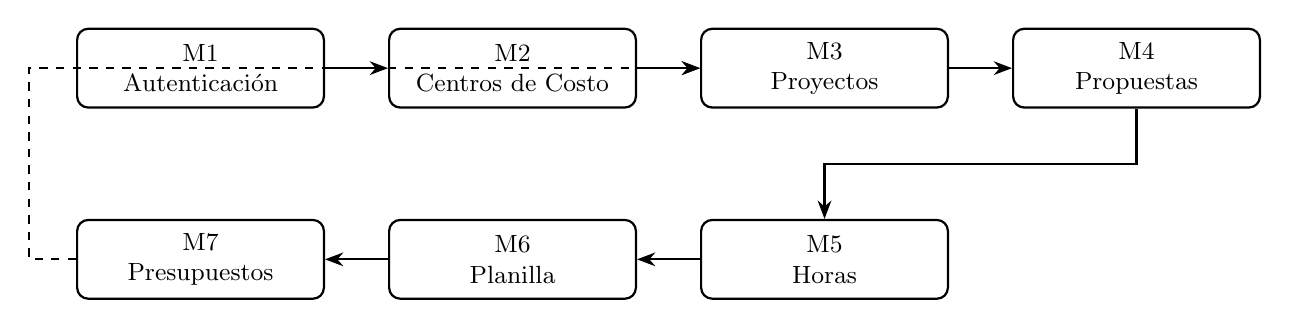
\begin{tikzpicture}[
  node distance=0.6cm and 0.8cm,
  box/.style={rectangle, rounded corners=4pt, draw, thick,
              text width=2.9cm, minimum height=1.0cm,
              align=center, font=\small},
  arr/.style={-{Stealth}, thick},
]
% Fila superior
\node[box] (auth)     {M1\\Autenticación};
\node[box, right=of auth]  (cc)   {M2\\Centros de Costo};
\node[box, right=of cc]    (proy) {M3\\Proyectos};
\node[box, right=of proy]  (prop) {M4\\Propuestas};
% Fila inferior
\node[box, below=1.4cm of auth]   (pres) {M7\\Presupuestos};
\node[box, right=of pres]         (plan) {M6\\Planilla};
\node[box, right=of plan]         (hs)   {M5\\Horas};
% Flechas fila superior
\draw[arr] (auth) -- (cc);
\draw[arr] (cc)   -- (proy);
\draw[arr] (proy) -- (prop);
% Flecha columna derecha
\draw[arr] (prop.south) -- ++(0,-0.7) -| (hs.north);
% Flechas fila inferior (derecha a izquierda)
\draw[arr] (hs)   -- (plan);
\draw[arr] (plan) -- (pres);
% Retroalimentación de presupuesto a proyectos
\draw[arr, dashed] (pres.west) -- ++(-0.6,0) |- (proy.west);
\end{tikzpicture}
\caption{Flujo de dependencias entre los módulos del sistema ERP. La flecha punteada indica que los datos de presupuesto retroalimentan la vista financiera del módulo de proyectos.}
\fuente{Elaboración propia, 2026.}
\end{figure}

El diseño del modelo de datos incluye adicionalmente las entidades necesarias para los módulos fuera del alcance del presente proyecto de grado —Requisiciones y Compras, Viáticos, Certificación Planificada y Tablero de Comando Gerencial—, garantizando que la arquitectura de datos soporte la evolución futura del sistema sin necesidad de reestructurar el esquema existente.

% =============================================================================
% 7. DISEÑO METODOLÓGICO
% =============================================================================
\section{Diseño Metodológico}

El proyecto adopta una metodología de desarrollo iterativa e incremental, organizada en fases al final de las cuales se entrega funcionalidad real y demostrable, validada con usuarios reales de ISI Mustang Bolivia. La validación es de dos tipos: técnica, verificando que el sistema produce los comportamientos especificados en los FRDs de manera consistente; y de usuario, verificando que los flujos de trabajo son comprensibles y utilizables por el personal de la empresa.

\subsection{Tipo de Investigación}

El presente trabajo es una investigación aplicada de tipo descriptivo-propositivo: describe el problema existente en el sistema de gestión actual de ISI Mustang Bolivia y propone una solución tecnológica concreta que se implementa y valida. El enfoque es mixto: cuantitativo en la medición del comportamiento del sistema —tiempos de respuesta, tasas de error, cobertura de pruebas, cumplimiento de requerimientos funcionales— y cualitativo en la validación de la experiencia del usuario durante las pruebas de aceptación con personal de la empresa \parencite{pressman2014}.

\subsection{Método de Investigación}

Se aplica una metodología iterativa e incremental basada en los principios de Scrum, adaptada al contexto de la organización \parencite{larman2004}. Cada sprint tiene una duración de dos semanas. Los artefactos del proceso incluyen: el Product Backlog con los requerimientos priorizados de todos los módulos; el Sprint Backlog con los requerimientos del sprint en curso; y el Documento de Requerimientos Funcionales por módulo como especificación formal previa al inicio del desarrollo \parencite{wiegers2013}. Las ceremonias del proceso comprenden la planificación del sprint, la demostración al final de cada iteración con validación de usuarios de ISI Mustang, y la retrospectiva para incorporar mejoras al proceso.

\subsection{Técnicas e Instrumentos de Investigación}

\subsubsection{Técnicas}

Se utilizan entrevistas estructuradas con usuarios clave de ISI Mustang Bolivia —gerencia, administración y empleados operativos— para el relevamiento de requerimientos. Se realiza análisis documental del sistema actual mediante el estudio de pantallas, reportes y flujos de trabajo existentes. Se aplica observación directa de los procesos operativos en la empresa para contrastar la documentación disponible con la práctica real. Se emplea prototipado iterativo con mockups validados por los usuarios antes de cada fase de implementación. Se ejecutan pruebas funcionales por módulo contra los FRDs correspondientes y pruebas de integración que verifican el flujo de negocio de extremo a extremo.

\subsubsection{Instrumentos}

Los instrumentos correspondientes a cada técnica son los siguientes: guías de entrevista semiestructurada para el relevamiento de requerimientos con usuarios clave; cuestionarios de aceptación de usuario para la validación del sistema en ambiente real; FRDs por módulo como instrumento central de especificación y verificación funcional; matrices de análisis comparativo para la evaluación de soluciones ERP existentes respecto al sistema propuesto; y el diagrama de entidad-relación como instrumento de diseño y verificación del modelo de datos.

\subsection{Población y Muestra}

La población objetivo son las empresas de consultoría e ingeniería de proyectos de tamaño medio en Bolivia que operan con sistemas de gestión obsoletos. La fuente primaria de información son los usuarios de ISI Mustang Bolivia, consultados mediante entrevistas estructuradas durante el relevamiento de requerimientos y mediante pruebas de aceptación durante la validación final. Las fuentes secundarias incluyen la documentación técnica oficial de NestJS, PostgreSQL, React y Prisma, la literatura académica sobre arquitectura de software y sistemas ERP, y el análisis de soluciones comerciales existentes como SAP, Oracle ERP Cloud y Odoo. La muestra para la validación con usuarios se selecciona por conveniencia, dado el carácter aplicado de la investigación y el acceso disponible al personal de ISI Mustang Bolivia.

% =============================================================================
% 8. ÍNDICE TENTATIVO
% =============================================================================
\section{Índice Tentativo}

\begin{indicetentativo}
INTRODUCCIÓN \\[2pt]
CAPÍTULO I. MARCO GENERAL \\
\quad 1.1 Antecedentes \\
\quad 1.2 Planteamiento del Problema \\
\quad\quad 1.2.1 Formulación del Problema \\
\quad\quad 1.2.2 Árbol del Problema \\
\quad 1.3 Objetivos \\
\quad\quad 1.3.1 Objetivo General \\
\quad\quad 1.3.2 Objetivos Específicos \\
\quad 1.4 Justificación \\
\quad\quad 1.4.1 Justificación Práctica \\
\quad\quad 1.4.2 Justificación Técnica \\
\quad\quad 1.4.3 Justificación Académica \\
\quad 1.5 Delimitación de la Investigación \\
\quad\quad 1.5.1 Delimitación Temática \\
\quad\quad 1.5.2 Delimitación Espacial \\
\quad\quad 1.5.3 Delimitación Temporal \\
\quad 1.6 Metodología \\
\quad\quad 1.6.1 Tipo de Investigación \\
\quad\quad 1.6.2 Método de Investigación \\
\quad\quad 1.6.3 Técnicas e Instrumentos de Investigación \\
\quad\quad 1.6.4 Fuentes de Información \\
\quad\quad 1.6.5 Propuesta de Solución \\[2pt]
CAPÍTULO II. MARCO TEÓRICO Y TECNOLÓGICO \\
\quad 2.1 Sistemas de Planificación de Recursos Empresariales \\
\quad\quad 2.1.1 Definición y Evolución de los Sistemas ERP \\
\quad\quad 2.1.2 Módulos Funcionales y Arquitectura Modular en ERP \\
\quad\quad 2.1.3 ERP para Empresas de Proyectos de Ingeniería \\
\quad\quad 2.1.4 Análisis Comparativo de Soluciones ERP Existentes \\
\quad 2.2 Arquitectura de Software \\
\quad\quad 2.2.1 Arquitectura Monolítica Modular \\
\quad\quad 2.2.2 Separación por Dominios Funcionales \\
\quad\quad 2.2.3 Arquitectura Limpia y Patrones de Diseño SOLID \\
\quad\quad 2.2.4 Modelo C4 para Documentación de Arquitectura \\
\quad 2.3 Tecnologías de Desarrollo \\
\quad\quad 2.3.1 NestJS como Framework de Backend \\
\quad\quad 2.3.2 PostgreSQL: Tipos Avanzados, Triggers y Row-Level Security \\
\quad\quad 2.3.3 Prisma como ORM y Gestor de Migraciones \\
\quad\quad 2.3.4 React y TailwindCSS para el Frontend \\
\quad\quad 2.3.5 JWT y Gestión de Sesiones \\
\quad 2.4 Metodología y Especificación de Requerimientos \\
\quad\quad 2.4.1 Desarrollo Iterativo e Incremental \\
\quad\quad 2.4.2 Scrum como Marco de Trabajo \\
\quad\quad 2.4.3 Documento de Requerimientos Funcionales (FRD) \\
\quad\quad 2.4.4 Pruebas de Software: Funcionales, de Integración y de Aceptación \\[2pt]
CAPÍTULO III. ANÁLISIS Y DISEÑO DEL SISTEMA PROPUESTO \\
\quad 3.1 Análisis del Sistema Actual de ISI Mustang \\
\quad 3.2 Requerimientos Funcionales y No Funcionales \\
\quad 3.3 Modelo de Datos: Diagrama Entidad-Relación \\
\quad 3.4 Diseño de la Arquitectura del Sistema \\
\quad 3.5 Diseño de Módulos y Flujos de Trabajo \\
\quad\quad 3.5.1 Módulo de Autenticación y Control de Acceso \\
\quad\quad 3.5.2 Módulo de Centros de Costo \\
\quad\quad 3.5.3 Módulo de Proyectos y Clientes \\
\quad\quad 3.5.4 Módulo de Propuestas Comerciales \\
\quad\quad 3.5.5 Módulo de Gestión de Horas \\
\quad\quad 3.5.6 Módulo de Planilla de Personal \\
\quad\quad 3.5.7 Módulo de Presupuestos \\
\quad 3.6 Diseño de la Interfaz de Usuario \\
\quad 3.7 Plan de Desarrollo por Fases e Incrementos \\[2pt]
CAPÍTULO IV. CONSTRUCCIÓN E IMPLEMENTACIÓN DEL SISTEMA \\
\quad 4.1 Ambiente de Desarrollo e Infraestructura \\
\quad 4.2 Fase 0: Relevamiento y Definición \\
\quad 4.3 Fase 1: Fundación del Sistema \\
\quad\quad 4.3.1 Implementación de M1 — Autenticación \\
\quad\quad 4.3.2 Implementación de M2 — Centros de Costo \\
\quad\quad 4.3.3 Implementación de M3 — Proyectos y Clientes \\
\quad 4.4 Fase 2: Personas y Pipeline Comercial \\
\quad\quad 4.4.1 Implementación de M4 — Propuestas Comerciales \\
\quad\quad 4.4.2 Implementación de M5 — Gestión de Horas \\
\quad\quad 4.4.3 Implementación de M6 — Planilla de Personal \\
\quad 4.5 Fase 3: Control Financiero \\
\quad\quad 4.5.1 Implementación de M7 — Presupuestos \\
\quad 4.6 Pruebas Funcionales e Integración End-to-End \\
\quad 4.7 Pruebas de Aceptación con Usuarios de ISI Mustang \\
\quad 4.8 Manual Técnico \\
\quad 4.9 Manual de Usuario \\[2pt]
CONCLUSIONES \\
RECOMENDACIONES \\
REFERENCIAS BIBLIOGRÁFICAS \\
ANEXOS
\end{indicetentativo}

% =============================================================================
% 9. MARCO TEÓRICO
% =============================================================================
\section{Marco Teórico}

Los fundamentos teóricos del presente trabajo se organizan en cuatro áreas: sistemas de planificación de recursos empresariales, arquitectura de software, tecnologías de desarrollo y metodología de construcción de sistemas. Estas áreas permiten justificar las decisiones de diseño del sistema propuesto y situar la contribución del proyecto en el contexto del conocimiento existente.

\subsection{Sistemas de Planificación de Recursos Empresariales}

Un ERP es un sistema de información integrado que centraliza los datos y procesos operativos de una organización en una plataforma única \parencite{monk2012}. Los sistemas ERP eliminan la duplicación de datos, garantizan consistencia entre departamentos y permiten reportes consolidados en tiempo real. Su arquitectura modular permite que un registro creado en un módulo —por ejemplo, un proyecto— sea inmediatamente visible y utilizable por todos los demás módulos del sistema, a diferencia de los sistemas aislados que requieren integración manual entre herramientas.

Los ERP diseñados para empresas de proyectos de ingeniería presentan requisitos específicos que los distinguen de los ERP genéricos: control de costos por proyecto, imputación de horas de trabajo a centros de costo, gestión de ciclos de aprobación para compras y gastos, y seguimiento del margen financiero por contrato activo. Estos requisitos determinan la estructura modular y la lógica de integración del sistema propuesto.

\subsection{Arquitectura Monolítica Modular y Separación por Dominios}

La arquitectura monolítica modular organiza una aplicación en módulos internos con límites claros de responsabilidad, pero que se despliegan como una única unidad \parencite{newman2021}. Cada módulo expone una interfaz pública y oculta sus detalles de implementación, de manera que los cambios internos de un módulo no afectan a los demás mientras la interfaz se mantenga estable. Esta arquitectura es preferible a los microservicios en las etapas iniciales de un sistema porque reduce la complejidad operacional al mantener un solo proceso a monitorear y desplegar, facilita la refactorización temprana sin la sobrecarga de comunicación entre servicios, y permite evolucionar a microservicios extrayendo módulos maduros cuando la escala del sistema lo justifique.

\textcite{martin2017} plantea que la arquitectura limpia organiza el software en capas concéntricas donde las dependencias apuntan hacia el interior, separando las reglas de negocio puras de los mecanismos de entrega —controladores HTTP, adaptadores de base de datos, interfaces de usuario—. En el presente proyecto, esta separación se materializa en la distinción entre la lógica de dominio de cada módulo NestJS y los controladores que exponen sus servicios mediante una API REST. \textcite{fowler2002} amplía este enfoque describiendo patrones de arquitectura empresarial aplicables a sistemas de gestión organizacional, incluyendo el patrón de repositorio que encapsula el acceso a datos y el patrón de servicio de dominio que concentra la lógica de negocio.

\subsection{Tecnologías de Desarrollo}

NestJS es un framework de Node.js para construir aplicaciones de servidor eficientes y escalables, construido sobre TypeScript \parencite{nestjs2024}. Su sistema de módulos, proveedores e inyección de dependencias sigue los principios SOLID y se alinea directamente con la arquitectura de dominio separado del sistema ERP propuesto: cada dominio funcional —autenticación, centros de costo, proyectos, propuestas, horas, planilla, presupuestos— se implementa como un módulo NestJS independiente con sus propios controladores, servicios y repositorios.

PostgreSQL es un sistema de gestión de bases de datos relacional de código abierto con soporte para tipos de datos avanzados, funciones almacenadas, triggers y políticas de seguridad a nivel de fila \parencite{postgresql2024}. La implementación de reglas de negocio críticas directamente en la base de datos garantiza que las restricciones se apliquen independientemente del mecanismo de acceso al dato. En el presente proyecto, el control de períodos contables cerrados se implementa a nivel de base de datos para garantizar que ningún proceso —ni errores en la capa de aplicación ni accesos directos— pueda modificar datos históricos ya cerrados.

\subsection{Metodología Iterativa e Incremental y Requerimientos Funcionales}

La metodología iterativa e incremental organiza el desarrollo en ciclos cortos al final de los cuales se entrega funcionalidad real y demostrable \parencite{larman2004}. Cada iteración incluye análisis, diseño, implementación y prueba de un subconjunto de requerimientos. Este enfoque es apropiado para el presente proyecto porque los requerimientos del sistema se conocen parcialmente desde el inicio y se refinan durante el relevamiento, y porque permite a los usuarios finales de ISI Mustang Bolivia validar funcionalidades reales antes de que el sistema completo esté terminado, reduciendo el riesgo de que el sistema entregado no responda a las necesidades reales del negocio.

El Documento de Requerimientos Funcionales especifica con precisión el comportamiento esperado de un módulo de software desde la perspectiva del usuario \parencite{wiegers2013}. Un FRD bien redactado incluye casos de uso, reglas de negocio, validaciones, restricciones y flujos alternativos. En el presente proyecto, se elaboraron FRDs durante la fase de relevamiento inicial para los módulos de Autenticación, Centros de Costo y Proyectos/Clientes; los módulos adicionales incluidos en el alcance contarán con su FRD antes del inicio del desarrollo correspondiente, siguiendo el mismo estándar de especificación.

% =============================================================================
% 10. CRONOGRAMA
% =============================================================================
\section{Cronograma}

El desarrollo del proyecto se organiza en cuatro fases durante la gestión 2026, con una duración total estimada de veinticuatro semanas. Cada fase entrega un subconjunto de módulos funcionales validados que se integra con los desarrollados en las fases anteriores. Los tiempos indicados son estimaciones; la fecha de inicio de la Fase 1 depende de la aprobación del anteproyecto y la disponibilidad horaria del postulante.

\begin{table}[H]
\centering
\caption{Cronograma de desarrollo por fases — gestión 2026.}
\begin{tabular}{p{0.06\textwidth}p{0.32\textwidth}p{0.18\textwidth}p{0.14\textwidth}p{0.14\textwidth}}
\toprule
\textbf{Fase} & \textbf{Actividades} & \textbf{Módulos} & \textbf{Semana inicio} & \textbf{Duración} \\
\midrule
0 & Relevamiento final, FRDs restantes, validación ERD & --- & 1 & 3 semanas \\
1 & Fundación del Sistema & M1, M2, M3 & 4 & 6 semanas \\
2 & Personas y Pipeline Comercial & M4, M5, M6 & 11 & 8 semanas \\
3 & Control Financiero & M7 & 20 & 4 semanas \\
--- & Testing y validación con usuarios & --- & 23 & 3 semanas \\
\bottomrule
\end{tabular}
\fuente{Elaboración propia, 2026.}
\end{table}

% =============================================================================
% 11. PRESUPUESTO ESTIMADO
% =============================================================================
\section{Presupuesto Estimado}

\begin{table}[H]
\centering
\caption{Presupuesto estimado del proyecto de grado.}
\begin{tabular}{p{0.38\textwidth}p{0.40\textwidth}p{0.12\textwidth}}
\toprule
\textbf{Ítem} & \textbf{Descripción} & \textbf{Costo (Bs.)} \\
\midrule
Equipamiento & Computadora de desarrollo (equipo propio) & 0 \\
Software y herramientas & Todas las herramientas son de código abierto y gratuitas & 0 \\
Infraestructura de desarrollo & PostgreSQL + NestJS en entorno local & 0 \\
Infraestructura de pruebas & Servidor de testing a cargo de ISI Mustang Bolivia & --- \\
Material bibliográfico & Libros, artículos y acceso a publicaciones académicas & 200 \\
Impresión y empastado & Documento final de tesis & 300 \\
Transporte & Visitas a ISI Mustang para relevamiento y validación & 500 \\
\midrule
\textbf{Total} & & \textbf{$\sim$1.000} \\
\bottomrule
\end{tabular}
\fuente{Elaboración propia, 2026.}
\end{table}

% =============================================================================
% 12. REFERENCIAS BIBLIOGRÁFICAS
% =============================================================================
\referencias

% =============================================================================
% ANEXOS
% =============================================================================
\seccioncuerpo{ANEXOS}

\end{document}
